\documentclass[border=0pt]{standalone}
\usepackage{tikz}
\usetikzlibrary{arrows}
\renewcommand\rmdefault{\sfdefault}

% define simple color names for esa colors and a highlight
\definecolor{esa}{RGB}{10,156,215}
\def\esacolorfactor{20}
\colorlet{esa0}{esa!90!white}
\colorlet{esa1}{black!\esacolorfactor!esa0}
\colorlet{esa2}{black!\esacolorfactor!esa1}
\colorlet{esa3}{black!\esacolorfactor!esa2}
\colorlet{esa4}{black!\esacolorfactor!esa3}
\colorlet{esa5}{black!\esacolorfactor!esa4}
\definecolor{highlight}{RGB}{189,27,27}



\begin{document}
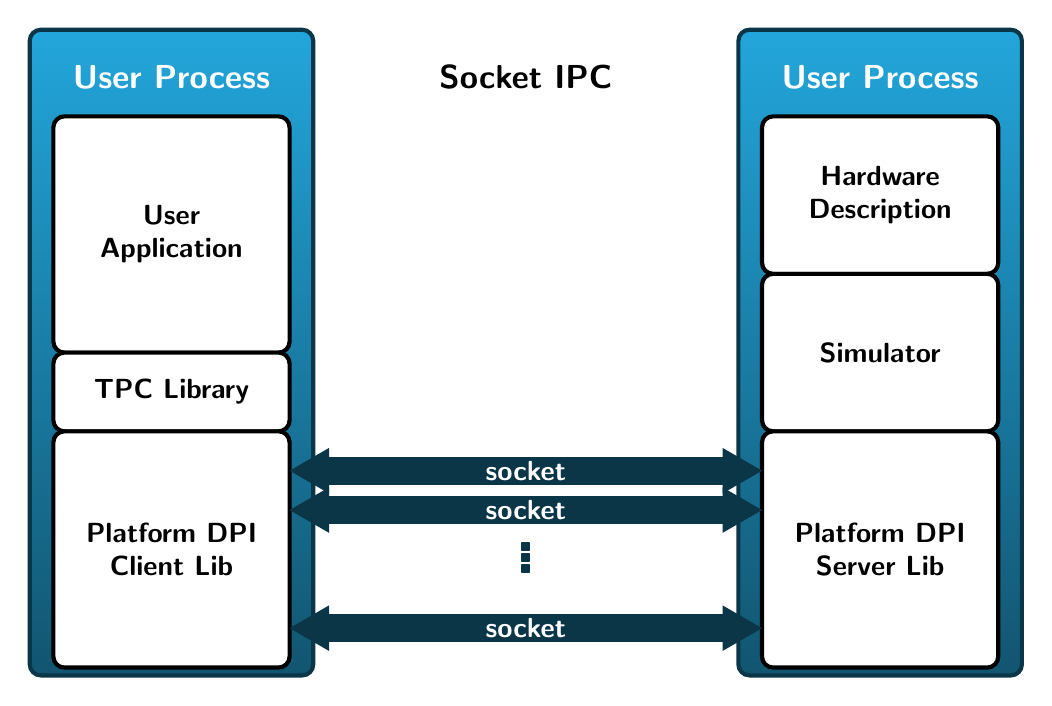
\begin{tikzpicture} [
    line width=1.5pt,
    y=-1cm, x=3cm, rounded corners,
    every node/.append style={align=center, font=\bfseries},
    process background/.style={top color=esa0, bottom color=esa3, draw=esa5, fill=esa3}
  ]

  \path [process background] (-.1, -1.1) rectangle (1.1, 7.1);
  \node [font=\bfseries\large\color{white}] at (0.5, -.5) {User Process};
  \begin{scope} [every path/.style={fill=white}]
    \draw (0,0) rectangle (1,3) node [pos=0.5] {User\\Application};
    %\draw (0,2) rectangle (1,3) node [pos=0.5] {FastFlow};
    \draw (0,3) rectangle (1,4) node [pos=0.5] {TPC Library};
    \draw (0,4) rectangle (1,7) node [pos=0.5] {Platform DPI\\Client Lib};
  \end{scope}

  \path [process background] (2.9, -1.1) rectangle (4.1, 7.1);
  \node [font=\bfseries\large\color{white}] at (3.5, -.5) {User Process};
  \begin{scope} [every path/.style={fill=white}]
    \draw (3,0) rectangle (4,2) node [pos=0.5] {Hardware\\Description};
    \draw (3,2) rectangle (4,4) node [pos=0.5] {Simulator};
    \draw (3,4) rectangle (4,7) node [pos=0.5] {Platform DPI\\Server Lib};
  \end{scope}

  \node [font=\bfseries\large] at (2, -.5) {Socket IPC};

  \begin{scope} [arr/.style={
      draw=esa5, fill=esa5, line width=3pt, <->, >=triangle 60,
      postaction={-, draw, line width=10pt, shorten >=12pt, shorten <=12pt}
      },
      every node/.style={font=\bfseries\color{white}}]
    \path [arr] (1,4.5) -- (3,4.5) node [pos=0.5] {socket};
    \path [arr] (1,5) -- (3,5) node [pos=0.5] {socket};
    \node [font=\bfseries\Huge\color{esa5}] at (2, 5.5) {\vdots};
    \path [arr] (1,6.5) -- (3,6.5) node [pos=0.5] {socket};
  \end{scope}
\end{tikzpicture}
\end{document}
